\documentclass[paper=a4, fontsize=12pt]{scrartcl}

\usepackage{graphicx}
\usepackage{siunitx}
\usepackage{amsmath}
\usepackage{mathrsfs}
\usepackage{float}
\usepackage{subfig}
\graphicspath{{./img/}}

\title{
	\normalfont \normalsize
	\textsc{University of Ottawa} \\ [5pt]
	\huge Discrete-Velocity Scheme Project
}
\author{Mathieu Marchildon} % Your name
\date{\normalsize \today} % Today's date or a custom date


\begin{document}
\maketitle


\section*{Shock-Tube Problem}
For the initial conditions of the shock-tube we must select an appropriate velocity space.
This velocity space can be determined by observing the distribution function on each side of
the shock tube for both initial conditions.
The distribution function in velocity space can be determined by applying Maxwell-Boltzmann distribution
for various ranges in velocity space.
\[
        f = \frac{\rho}{m} \Big( \frac{\rho}{2 \pi p}\Big)^{\frac{1}{2}}e^{\frac{\rho}{2 p}(u-v)^2}
\]
\begin{figure}[H]%
    \centering
    \subfloat[Left initial conditions]{{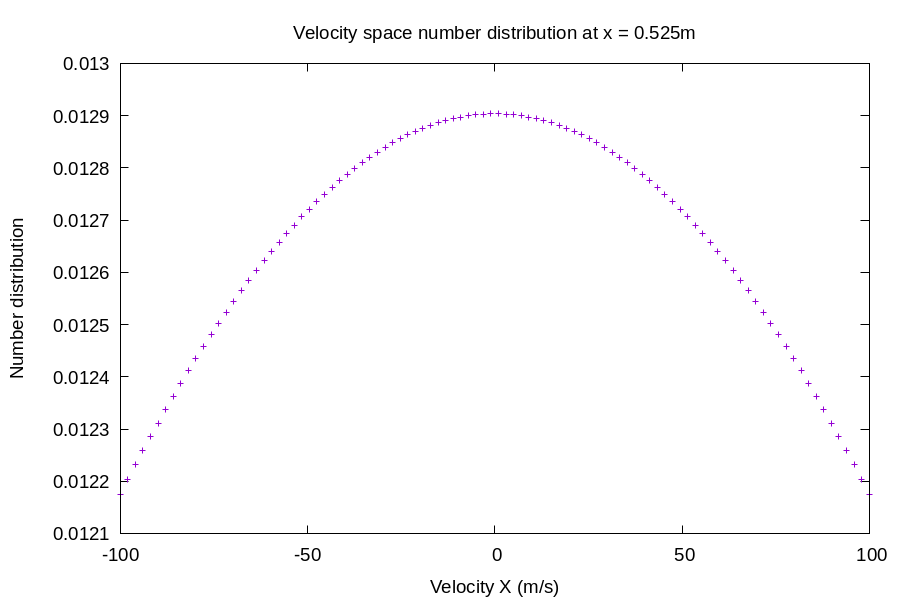
\includegraphics[width=7cm]{left_init_100} }}%
    \qquad
    \subfloat[Right initial conditions]{{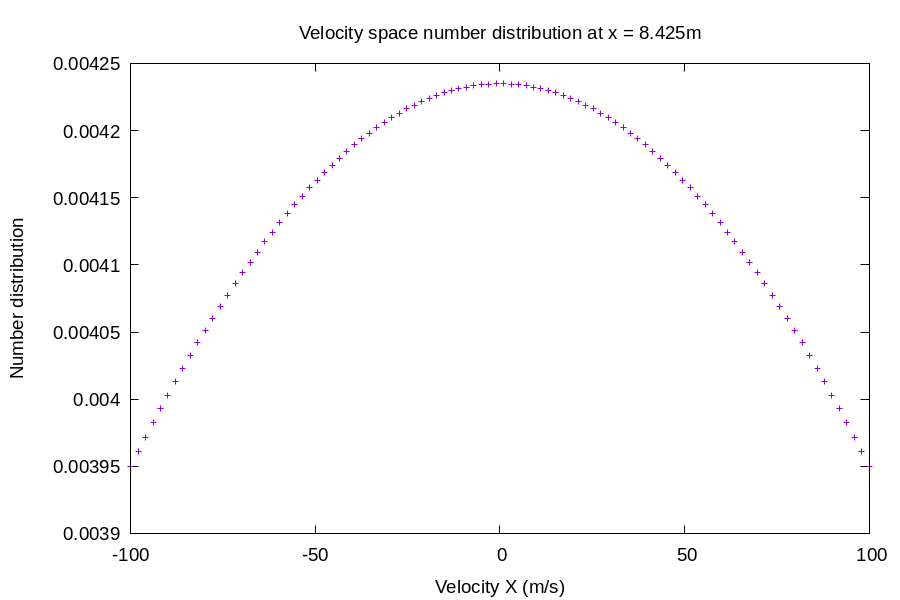
\includegraphics[width=7cm]{right_init_100} }}%
    \caption{Distribution function at initial conditions \newline velocity range of $\pm \SI{100}{\meter \per \second}$
 }
    \label{fig:init_100}%
\end{figure}

\noindent
Figure \ref{fig:init_100} shows the distribution function for the left and right initial conditions.
The velocity space selected was ranging from $\pm \SI{100}{\meter \per \second}$.
This range of velocity as shown in Figure \ref{fig:init_100} is insufficient as the tail
end of the distribution is cut off for both the left and right ends of the shock tubes.
\begin{figure}[H]
    \centering
    \subfloat[Left initial conditions]{{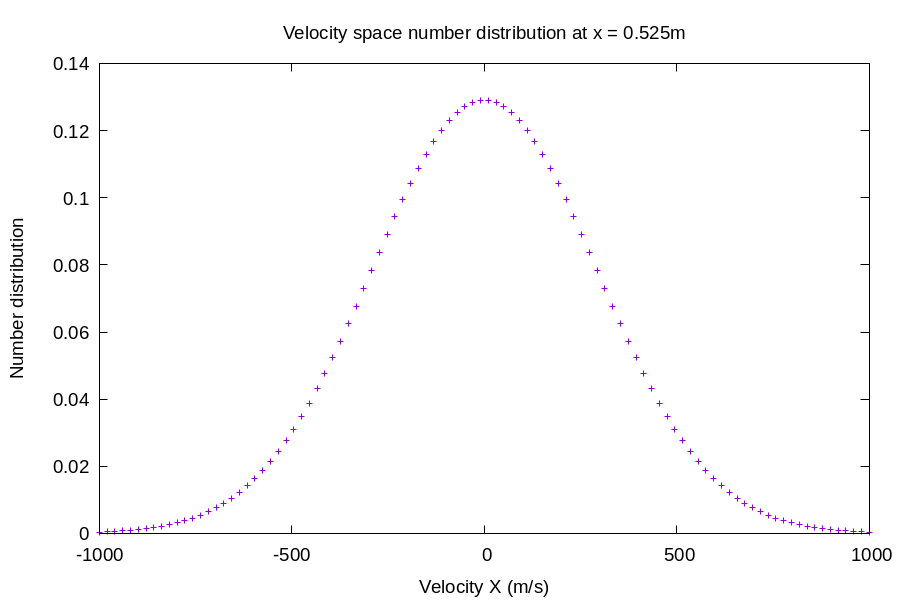
\includegraphics[width=7cm]{left_init_1000} }}%
    \qquad
    \subfloat[Right initial conditions]{{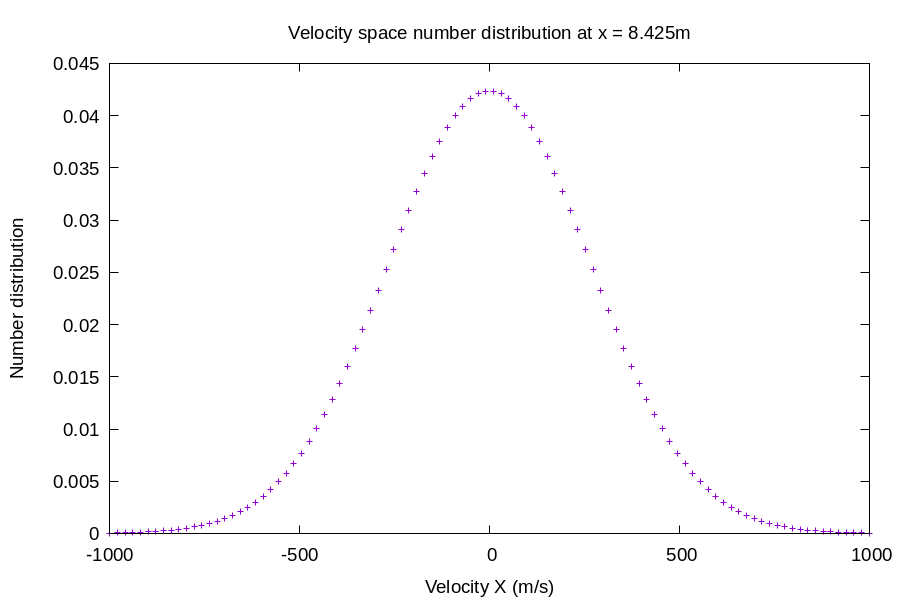
\includegraphics[width=7cm]{right_init_1000} }}%
    \caption{Distribution function at initial conditions \newline velocity range of $\pm \SI{1000}{\meter \per \second}$
 }
    \label{fig:init_1000}
\end{figure}

\noindent
Selecting a velocity range of $\pm \SI{1000}{\meter \per \second}$, as shown in \ref{fig:init_1000} we obtain
a velocity space that covers the full distribution of the particle space.


In addition to verifying the velocity space distribution we can also evaluate the properties of the gas
at those initial conditions.
The properties of the gas can be computed at each point in the $x$ direction by the following equations.

\begin{align*}
        \rho &= \langle m F \rangle  &  c = v-u\\
        \rho u &= \langle m v F \rangle \\
        p &= \langle m c^2 F \rangle \\
        q &= \frac{1}{2}\langle m c^3 F \rangle \\
\end{align*}

\begin{figure}[H]
    \centering
    \subfloat[Left initial conditions]{{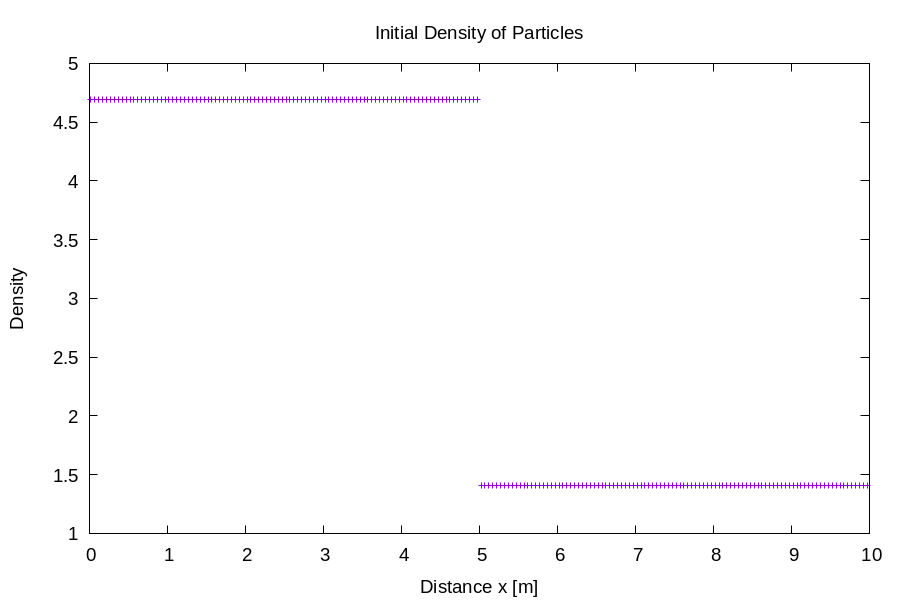
\includegraphics[width=7cm]{init-rho} }}%
    \qquad
    \subfloat[Right initial conditions]{{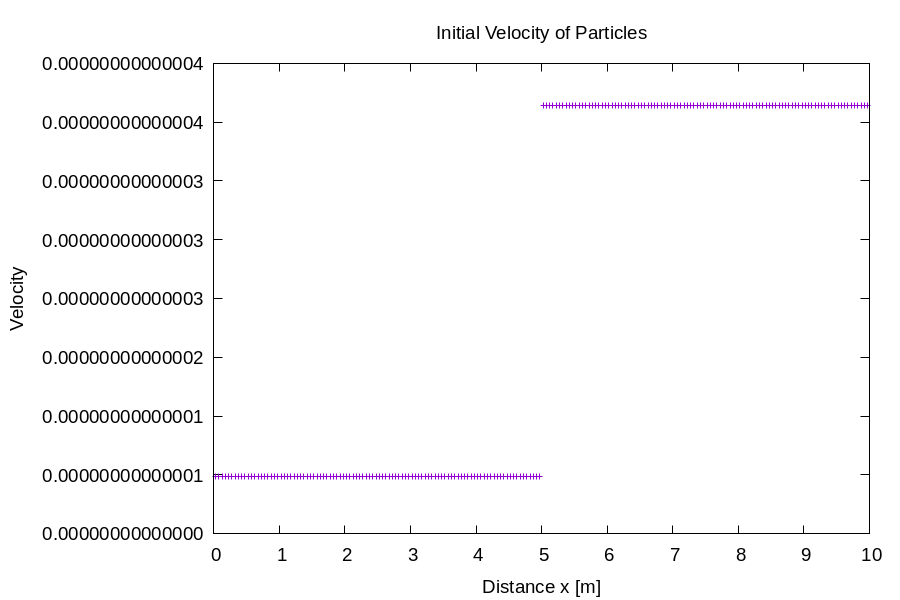
\includegraphics[width=7cm]{init-u} }}%
    \caption{Initial conditions $\rho,  u$
 }
    \label{fig:init-rho_u}
\end{figure}

\begin{figure}[H]
    \centering
    \subfloat[Left initial conditions]{{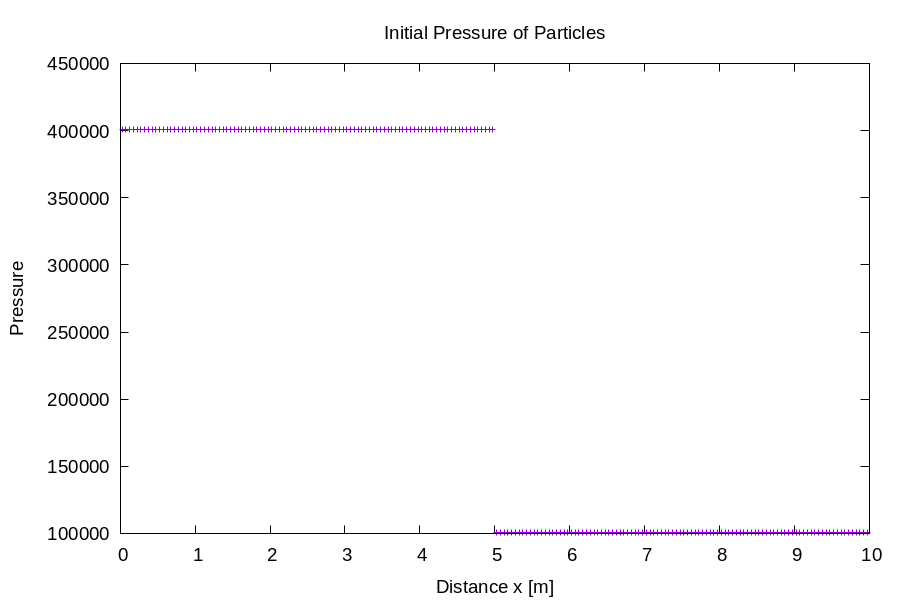
\includegraphics[width=7cm]{init-p} }}%
    \qquad
    \subfloat[Right initial conditions]{{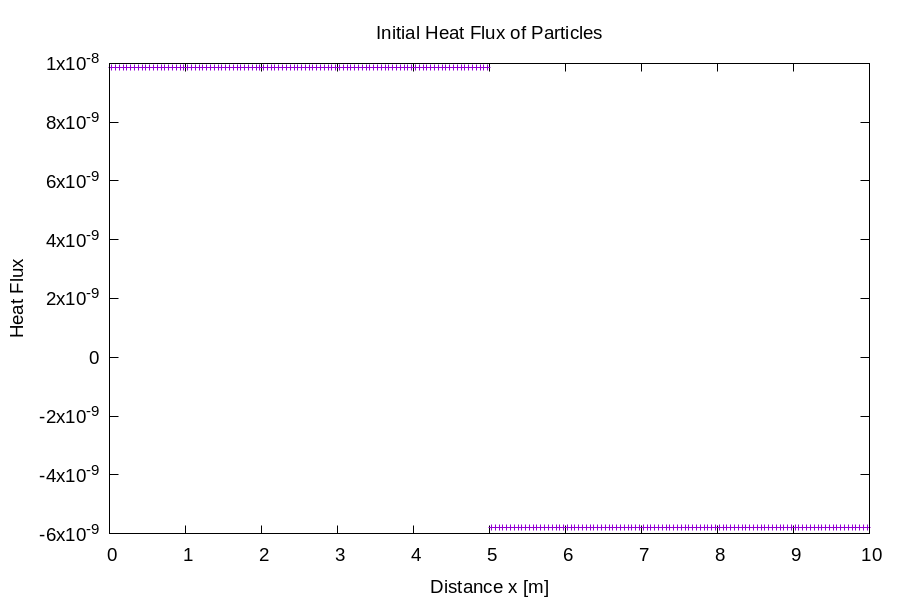
\includegraphics[width=7cm]{init-q} }}%
    \caption{Initial conditions $p, q$
 }
    \label{fig:init-p_q}
\end{figure}

\noindent
As shown in Figure \ref{fig:init-rho_u} and \ref{fig:init-p_q} the initial density calculated using the
set number density of the particles is around the $\SI{4.696}{\kilogram \per \meter^3}$
and $\SI{1.408}{\kilogram \per \meter^3}$.
The initial velocities and heat flux are near zero and the pressure is set to be near
$\SI{404.4}{\kilo \pascal}$ and $\SI{101.1}{\kilo \pascal}$.

\subsection*{Results}
\begin{figure}[H]
        \centering
        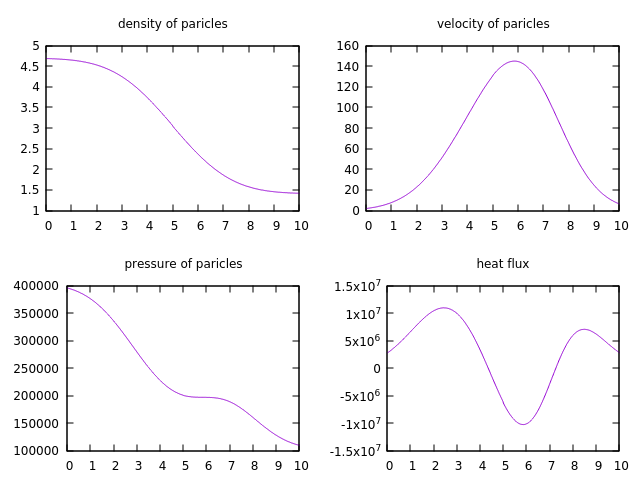
\includegraphics[width=0.8\textwidth]{tau10}
        \caption{$\tau$ = 10}
        \label{fig:tau10}
\end{figure}
\begin{figure}[H]
        \centering
        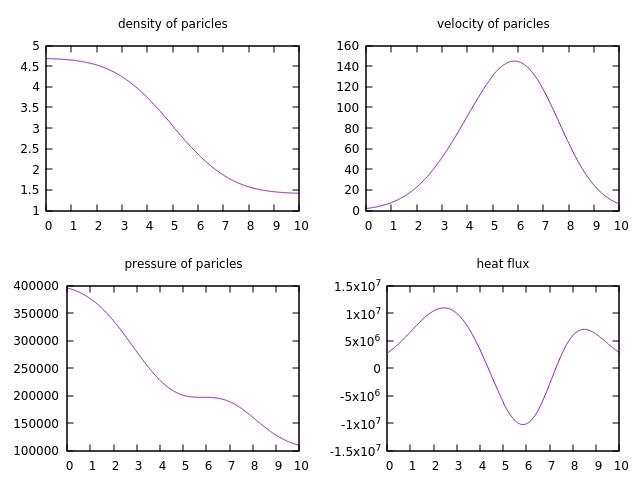
\includegraphics[width=0.8\textwidth]{tau1}
        \caption{$\tau$ = 1}
        \label{fig:tau1}
\end{figure}
\begin{figure}[H]
        \centering
        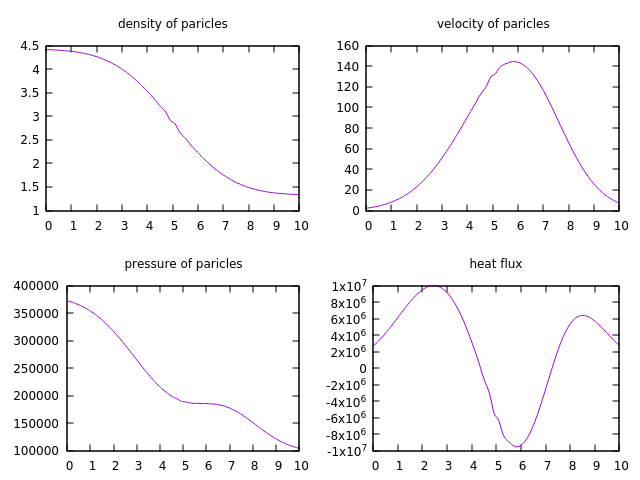
\includegraphics[width=0.8\textwidth]{tau0-1}
        \caption{$\tau$ = 0.1}
        \label{fig:tau0-1}
\end{figure}
\begin{figure}[H]
        \centering
        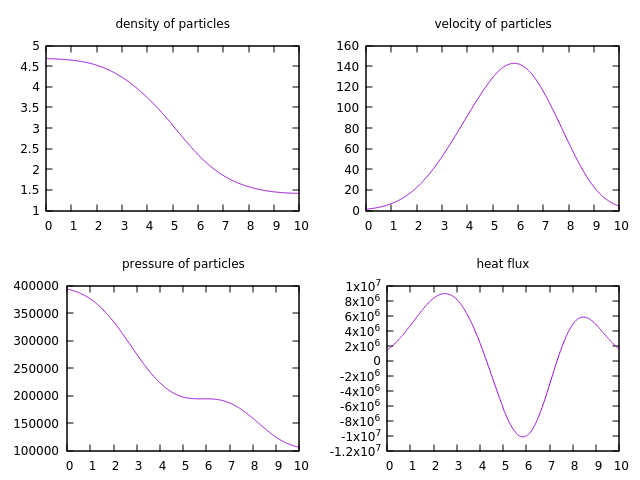
\includegraphics[width=0.8\textwidth]{tau0-01}
        \caption{$\tau$ = 0.01}
        \label{fig:tau0-01}
\end{figure}
\begin{figure}[H]
        \centering
        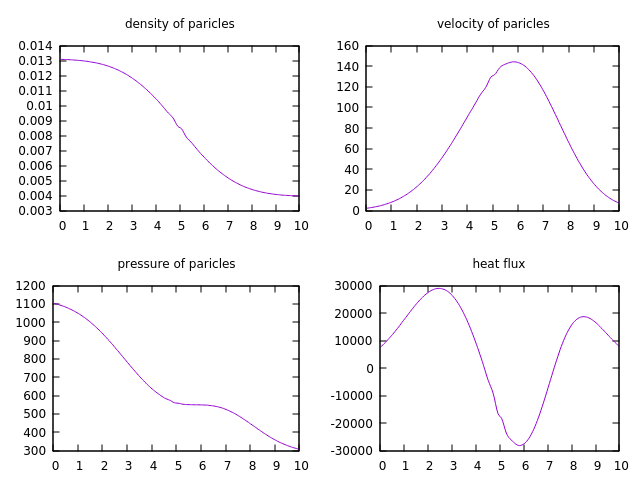
\includegraphics[width=0.8\textwidth]{tau0-001}
        \caption{$\tau$ = 0.001}
        \label{fig:tau0-001}
\end{figure}


\noindent
In addition to the change of the fluid properties along the $x$ axis we can also
evaluate the velocity distribution at certain points along the shock tube.
Looking at the probability distribution of the particles at given points lets us
observer the most likely velocities particles are to be found at those given points.

\begin{figure}[H]
        \centering
        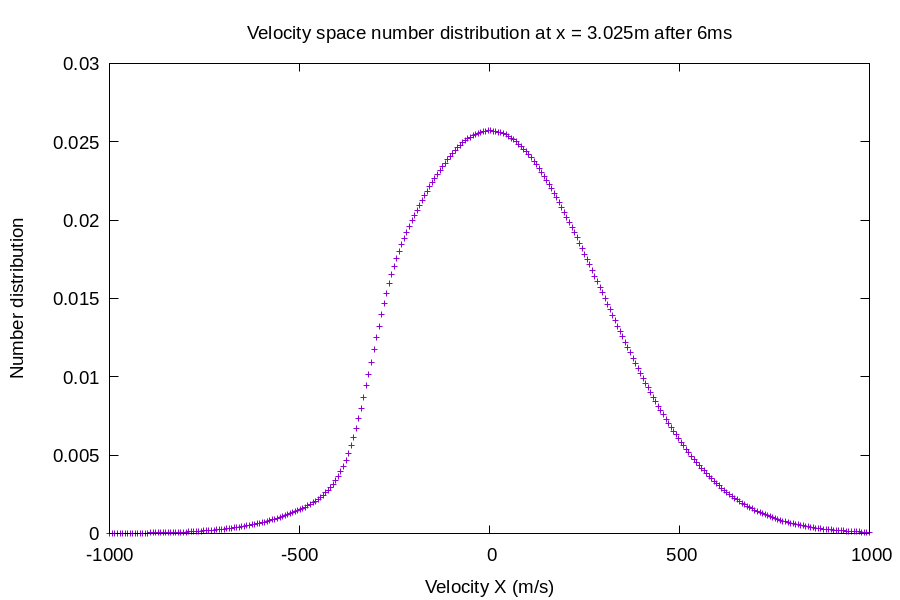
\includegraphics[width=0.8\textwidth]{left_f}
        \caption{Left velocity distribution at $x = \SI{3.025}{\meter}$ }
        \label{fig:left_f}
\end{figure}
\begin{figure}[H]
        \centering
        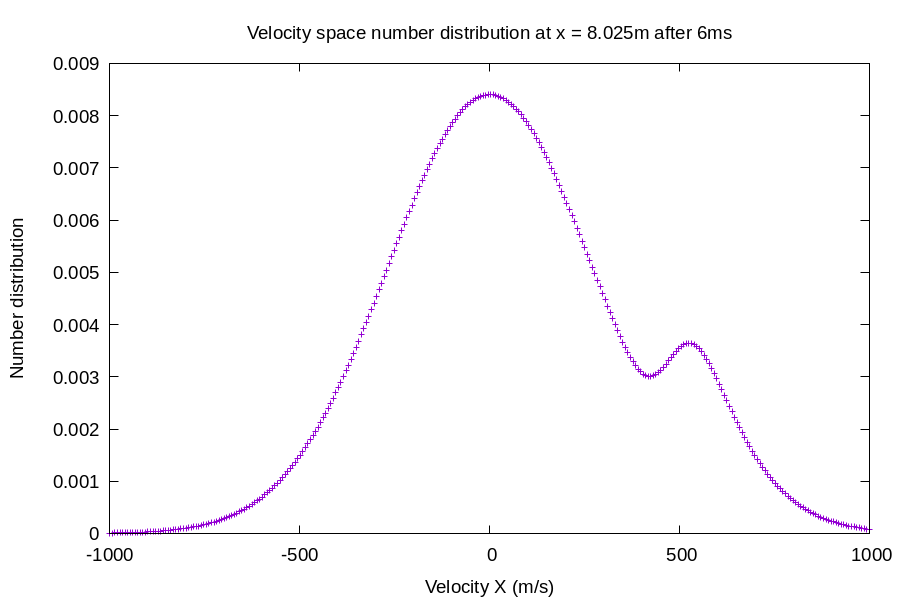
\includegraphics[width=0.8\textwidth]{right_f}
        \caption{Right velocity distribution at $x = \SI{8.025}{\meter}$ }
        \label{fig:right_f}
\end{figure}
\begin{figure}[H]
        \centering
        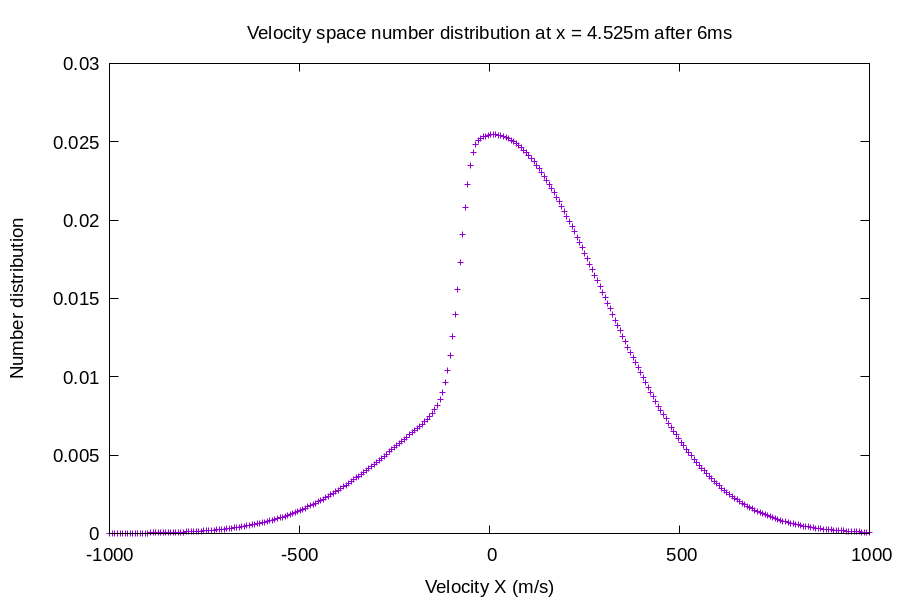
\includegraphics[width=0.8\textwidth]{center_shock}
        \caption{Velocity distribution near center of shock-tube}
        \label{fig:center_shock}
\end{figure}
\end{document}
